
This analysis uses several different control regions in addition to the signal regions. 
All of these different regions are defined in this section. 
Figure~\ref{fig:venndiagram} illustrates the relationship between these regions.

\subsection{Single Lepton Selections}

The single lepton preselection sample is based on the following criteria
\begin{itemize}
\item satisfy the trigger requirement (see
  Table.~\ref{tab:DatasetsData}). Dilepton triggers are used only for the dilepton control region.
\item select events with one high \pt\ electron or muon, requiring
  \begin{itemize}
  \item $\pt>30~\GeVc$ and $|\eta|<2.5(2.1)$ for \E(\M)
  \item satisfy the identification and isolation requirements detailed
    in the same-sign SUSY analysis (SUS-11-010) for electrons and the opposite-sign 
    SUSY analysis (SUS-11-011) for muons
  \end{itemize} 
  \item require at least 4 PF jets in the event with $\pt>30~\GeV$
    within $|\eta|<2.5$
  \item require moderate $\met>50~\GeV$
\end{itemize}

In addition, we count the number of SSV medium working point b-tags, $N_{b-tag}$.

Currently, we focus on the muon channel because it is cleaner (the QCD contribution is negligible)
and the triggers are simpler (we use single muon triggers, as opposed to electron + 3-jet triggers).
We will add the electron channel, time permitting. However, since this is a systematics-dominated 
analysis, increasing the statistics by adding the electrons is not expected to significantly improve
the sensitivity, especially because the electron selection efficiency is smaller and the systematic
uncertainty associated with the QCD background is larger.
    
We then define the following subsamples within this preselection sample:
\begin{itemize}
\item $N_{b-tag} = 0$, i.e. b-veto region
\item $N_{b-tag} \ge 1 $, i.e. b-tagged region
\begin{itemize}
\item without an additional isolated track veto
\item with an additional isolated track veto
\end{itemize}
\end{itemize}

For the signal regions, we then furthermore require $\met>100~\GeV$ while some of the background predictions and scale factors
are done for both \met
requirements to show stability of the method.
Within each of these subsamples we then define an \mt peak ($60 < \mt < 100~\GeV$) region and an \mt tail ($\mt > 150~\GeV$) region
%
We generally use the \mt peak region yields in data and multiply it by the ratio of tail divided by peak in MC times appropriate corrections
in order to estimate the background in data in the tail region.

{\bf We have not looked at the data in the signal region after the first 1 fb$^{-1}$ of data.}

\subsection{Dilepton control region}

We define a dilepton control region requiring two isolated leptons, $ee, e\mu$, or $\mu\mu$ to study the jet multiplicity in data and MC, and derive
scale factors based on their consistency. This study is documented in Section~\ref{sec:jetmultiplicity}.

{\bf Fix me: Need to describe here the actual selection. What lepton pT's, \met , etc. } 

This sample is only partially overlapping with the single lepton preselection as it requires the dilepton rather than the single lepton triggers.

\subsection{Corrections to Jets and \met}

The official recommendations from the Jet/MET group are used for 
the data and MC samples. In particular, the jet
energy corrections (JEC) are updated using the official recipe.
L1FastL2L3Residual (L1FastL2L3) corrections are applied for data (MC),
based on the global tags GR\_R\_42\_V23 (DESIGN42\_V17) for
data (MC). In addition, these jet energy corrections are propagated to
the \met\ calculation, following the official prescription for
deriving the Type I corrections. It may be noted that events with
anomalous ``rho'' pile-up corrections are excluded from the sample since these 
correspond to events with unphysically large \met\ and \mt\ tail
signal region (see Figure~\ref{fig:mtrhocomp}). An additional correction to remove
the $\phi$-modulation observed in the \met\ is included, improving 
the agreement between the data and the MC, as shown in 
Figure~\ref{fig:metphicomp}. This correction has an effect on this analysis,
since the azimuthal angle enters the \mt\ distribution. 

\clearpage

\begin{figure}[!ht]
  \begin{center}
	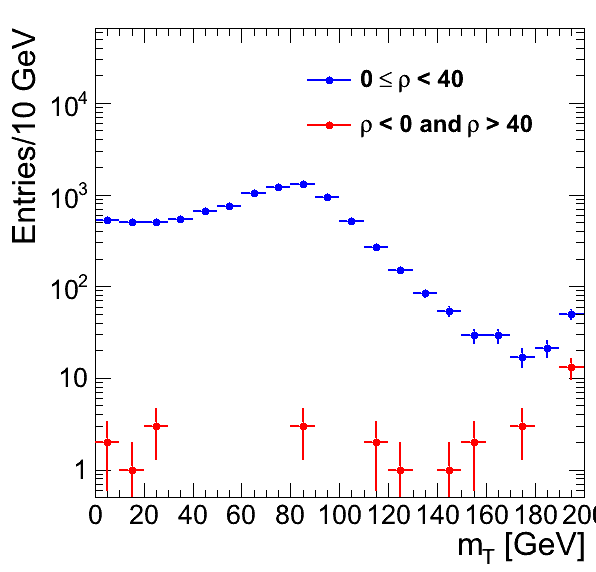
\includegraphics[width=0.5\linewidth]{plots/mt_rho_comp.png}
	\caption{ \label{fig:mtrhocomp}%\protect 
	  Comparison of the \mt\ distribution for events with
          unphysical energy corrections ($\rho <0$ or $ \rho > 40$, where $\rho$ is a
          measure of the average pileup energy density) and the
          nominal sample. Events with large pileup corrections 
          correspond to noisy events. Since this correction is applied
          to the jets and propagated to the \met, these events have
          anomalously large \met\ and populate the \mt\ tail. These
          pathological events are excluded from the analysis sample.}
  \end{center}
\end{figure}

\begin{figure}[!hb]
  \begin{center}
	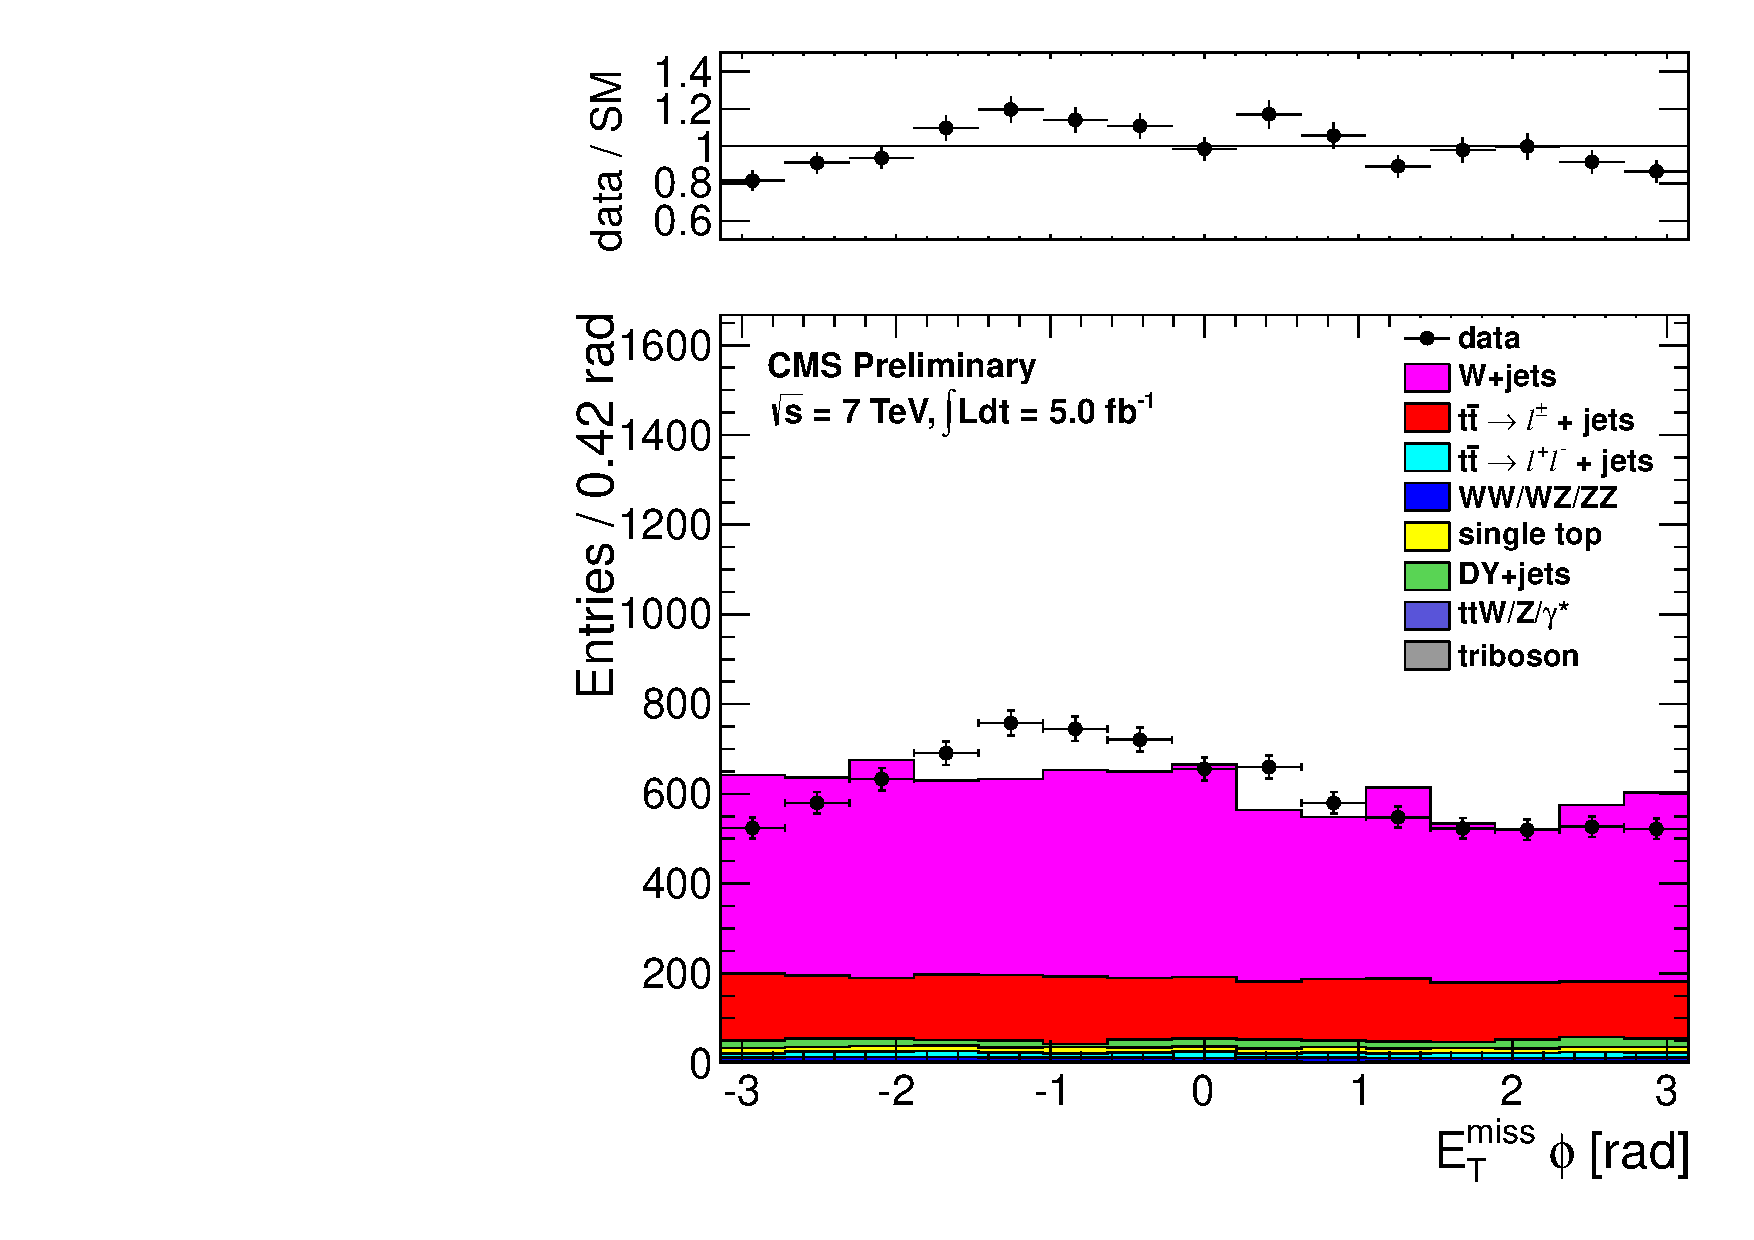
\includegraphics[width=0.5\linewidth]{plots/metphi.pdf}%
	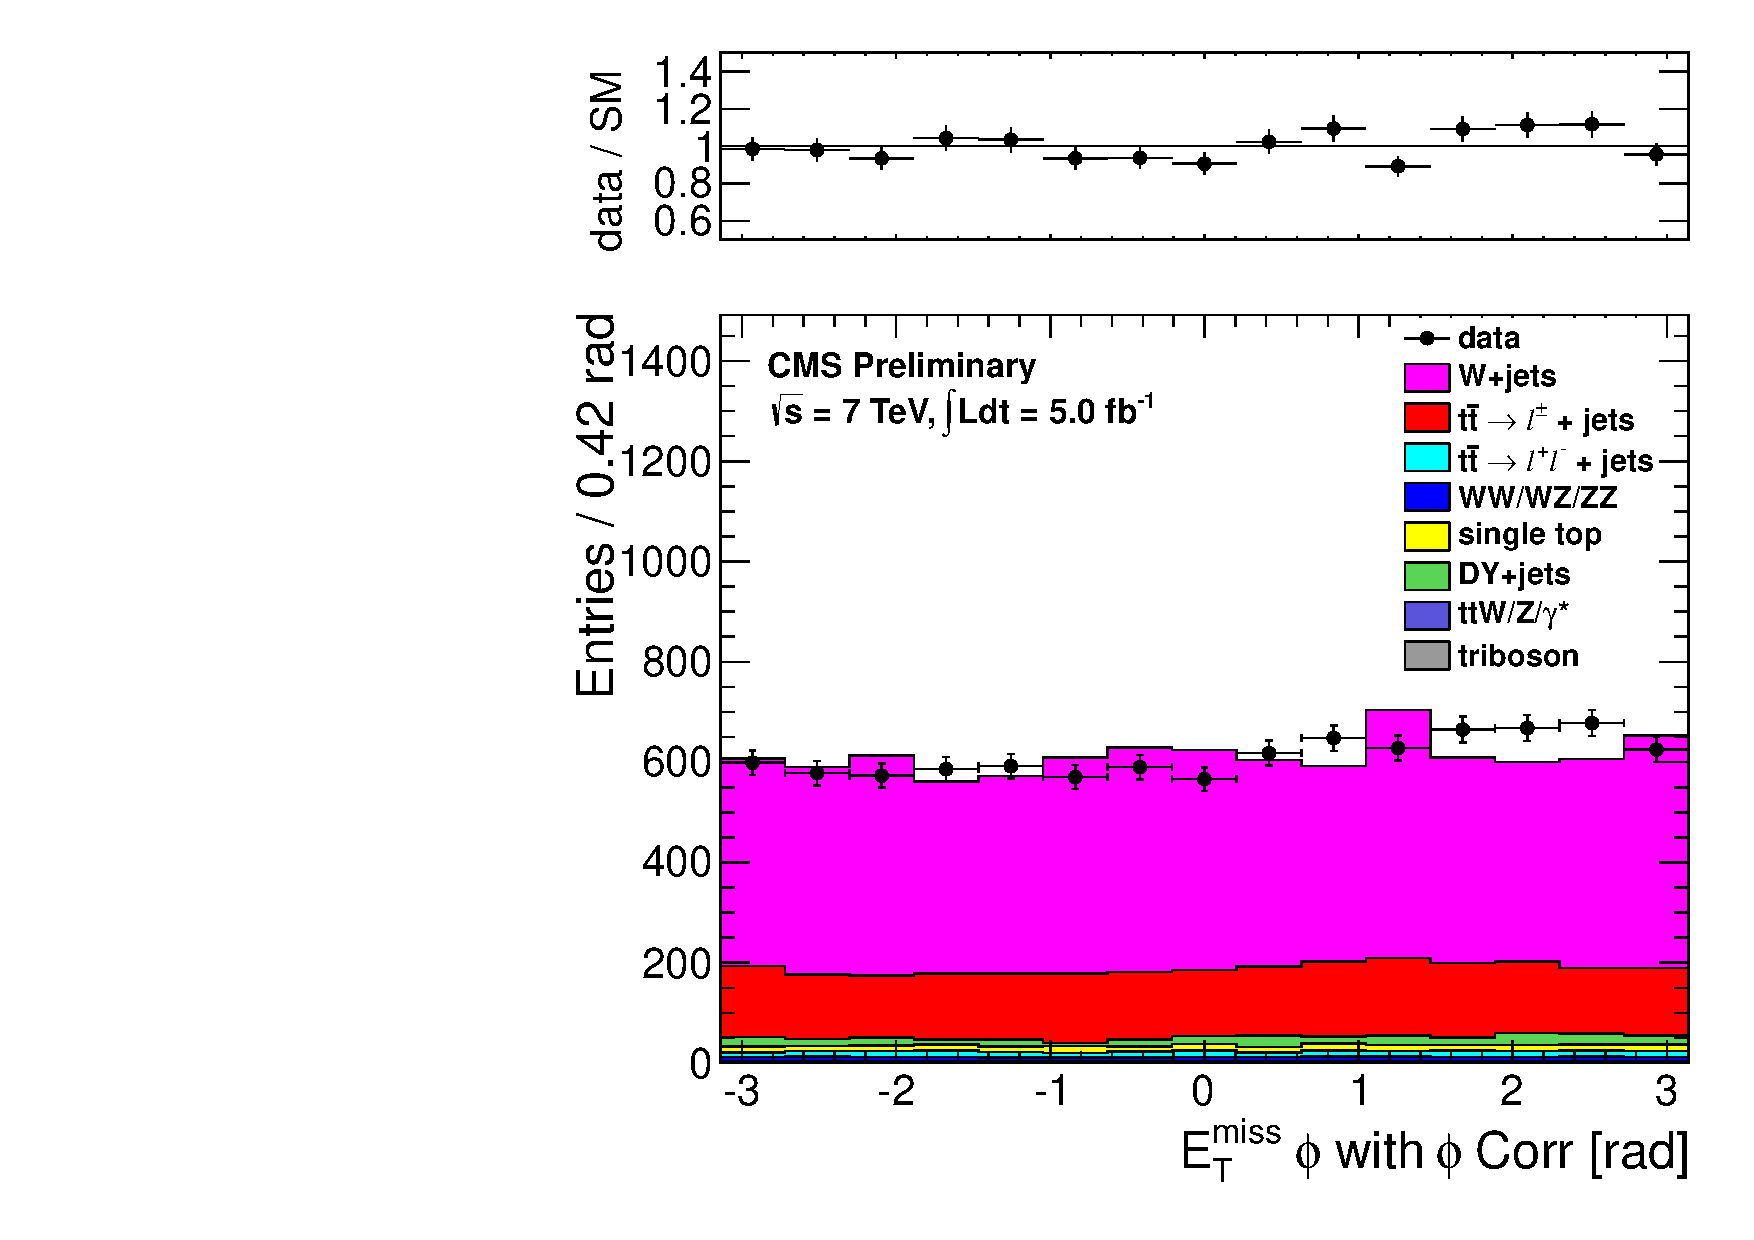
\includegraphics[width=0.5\linewidth]{plots/metphi_phicorr.pdf}
	\caption{ \label{fig:metphicomp}%\protect 
	  The PF \met\ $\phi$ distribution (left) exhibits a
          modulation. After applying a dedicated correction, the
          azimuthal dependence is reduced (right).}
  \end{center}
\end{figure}

\clearpage

\subsection{Branching Fraction Correction}

The leptonic branching fraction used in some of the \ttbar\ MC samples
differs from the value listed in the PDG $(10.80 \pm 0.09)\%$. 
Table.~\ref{tab:wlepbf} summarizes the branching fractions used in
the generation of the various \ttbar\ MC samples. 
For \ttbar\ samples with the incorrect leptonic branching fraction, event
weights are applied based on the number of true leptons and the ratio
of the corrected and incorrect branching fractions. 

\begin{table}[!h]
\begin{center}
\begin{tabular}{c|c}
\hline
         \ttbar\ Sample - Event Generator & Leptonic Branching Fraction\\
\hline
\hline
Madgraph   &       0.111\\
MC@NLO    &       0.111\\
Pythia         &       0.108\\
Powheg       &       0.108\\
\hline
\end{tabular}
\caption{Leptonic branching fractions for the various \ttbar\ samples
  used in the analysis. The primary \ttbar\ MC sample produced with
  Madgraph has a branching fraction that is almost $3\%$ higher than
  the PDG value. \label{tab:wlepbf}}
\end{center}
\end{table}

